
\chapter{Architettura e componenti Software}

\primalettera{P}er permettere al computer di bordo di inviare comandi
al drive e ricevere un feedback, � necessario trovare un modo di codificare
i messaggi ROS in CANframes.

Bench� la comunicazione non sia ancora possibile, in questo capitolo
si elencheranno i passaggi necessari ad eseguire il setup del drive,
dell'ambiente ROS, delle librerie e strumenti aggiuntivi necessari. 

\subsection{Setup drive }

I parametri statici che definiscono il funzionamento del drive devono
essere programmati attraverso una connessione seriale rs422, possibile
attraverso il convertitore moxa.

Per eseguire il setup del drive � stato necessario utilizzare Drive
Watcher, un software proprietario fornito dal produttore dei motori,
questa suite sfortunatamente � compatibile solo con windows xp e necessita
si un port non disponibile in una virtual machine il che rende impossibile
utilizzarla senza avere il sistema operativo installato. � stato quindi
necessario utilizzare una vecchio computer esclusivamente per programmare
i parametri del drive. 

\subsubsection{Abilitare Moxa}

Per abilitare il convertitore moxa � necessario per prima cosa installare
il driver da CD o file .zip della Moxa, il programma � presente all\textquoteright interno
della cartella riferita al convertitore Moxa che si possiede. Bisogna
entrare nella cartella Software, e installare file .exe. 

Per abilitare il port � necessario andare in Pannello di controllo
> Sistema > Hardware > Gestione Periferiche.
\begin{enumerate}
\item \begin{flushleft}
Da Porte (COM e LPT) cliccare col tasto destro su MOXA USB e aprire
Propriet�; in Port Settings impostare i seguenti valori : Baud Rate
= 9600, Data its = 8, Parity = None, Stop bits = 1, Flowcontrol =
None.
\begin{figure}[H]
\centering{}\includegraphics[scale=0.5]{\string"immagini/installazione moxa1\string".png}\caption{Installazione moxa, parte 1}
\end{figure}
\pagebreak{}
\par\end{flushleft}
\item \begin{flushleft}
Da Schede Seriali Multiport cliccare col tasto destro su Uport 1130I
e aprire Propriet�; in Ports Configuration aprire Port Setting della
COM in uso dalla Moxa e impostare : Fast Flush su Enable e Interface
su RS-422.
\begin{figure}[H]

\begin{centering}
\includegraphics[scale=0.5]{\string"immagini/installazione moxa2\string".png}\caption{Installazione moxa, parte2}
\par\end{centering}
\end{figure}
\par\end{flushleft}
\end{enumerate}

\subsection{Installazione Drive Watcher}

Per installare il software basta semplicemente estrarre e aprire il
file Setup-DriveWatcher-407.exe. 

Prima di modificare i parametri bisogna accertarsi che la moxa sia
connessa al driver e che la parte logica del driver sia alimentata
a 24V, con l'uscita negativa dell'alimentatore messa a terra. 

Si esegue un settaggio della comunicazione attraverso la modalit�
\textquotedbl{}Communication Settings\textquotedbl{}, impostando la
ComPort designata in precedenza e cercando il nodo attivo attraverso
il \textquotedbl{}search node tool\textquotedbl{}. L'ultimo tool menzionato
eseguir� uno sweep completo di tutti i nodi disponibili, indicando
quelli attivi con un colore differente. 

\begin{figure}[H]
\begin{centering}
\includegraphics[scale=0.5]{\string"immagini/node sweep\string".png}\caption{Communication Settings e Search Node Tool}
\par\end{centering}
\end{figure}

Una volta impostato il nodo si controlla che la connessione sia attiva
attraverso il tool \textquotedbl{}ComPort communication test\textquotedbl{}
(icona a cacciavite). 

\subsection{Programmazione dei parametri}

I parametri si possono visualizzare nella sezione \textquotedbl{}Parameters
configuration\textquotedbl{}, ogni parametro dispone di una descrizione
a lato, quindi in questo documento non si elencheranno tutti, ma solo
i pi� importanti ai fini del progetto. Per farsi un'idea pi� dettagliata
si possono consultare il manuale Siboni \textquotedbl{}Istruzioni
Drive Watcher\textquotedbl{} \cite{Siboni2018} e quello completo
del drive Microphase \textquotedbl{}Micro Digital One\textquotedbl{},
capitolo 9. \cite{Microphase}

\begin{figure}[H]

\begin{centering}
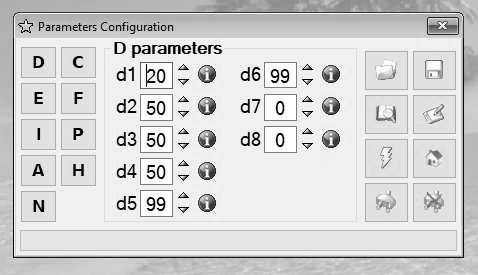
\includegraphics[scale=0.5]{immagini/parametri}\caption{lo strumento Parameters Configuration}
\par\end{centering}
\end{figure}
Fare particolare attenzione ai parametri: 
\begin{description}
\item [{C7}] numero nodo = 1 di default
\item [{C9}] modo di funzionamento del drive, impostato a 5 per il CANopen
\item [{D8}] selezione del motore utilizzato, nel nostro caso brushless
sinusoidale
\item [{N1}] bitrate CAN, impostiamo a 5 per 250Kbaud, 6 per 500Kbaud
\end{description}

\section{Setup ROS}

L'installazione di ROS varia in base alle release. In questo progetto
� stata utilizzata Melodic Morenia, ma in base alla distro di linux
installata sul computer di bordo potrebbe essere necessario installare
una release differente. Ritenendo inutile descrivere il processo di
installazione di una singola versione quando � disponibile online
ampia documentazione a riguardo, si include qui il link al sito ufficiale
di ROS, dove sono indicati tutti gli step necessari per le varie piattaforme:
\url{https://wiki.ros.org/ROS/Installation}.

Successivamente, si utilizza Catkin per creare un workspace in cui
sviluppare il progetto:

\begin{lstlisting}
$ mkdir -p ~/catkin_ws/src 
$ cd ~/catkin_ws/ 
$ catkin_make
\end{lstlisting}

Per rendere utilizzabili con roscd e roslaunch i pacchetti aggiuntivi
che installeremo nel workspace, � necessario aggiungere all'origine
il nuovo file setup.{*}sh

Dall'interno della cartella catkin\_ws, si scrive nel terminale:

\begin{lstlisting}
$ source devel/setup.bash
$ echo $ROS_PACKAGE_PATH /home/youruser/catkin_ws/src:/opt/ros/kinetic/share
\end{lstlisting}

Questo comando, insieme a catkin\_make, andr� ripetuto per sicurezza
ad ogni utilizzo del workspace e soprattuto dopo l'installazione di
nuovi pacchetti. 

\section{Setup PCAN}

Bench� dei driver per adattatore PCAN siano installati di default
nel kernel linux, per cui i canali CAN sono gestiti come dispositivi
netdev, per utilizzare il software di visualizzazione pcan\_view e
l'API pcan\_basic � necessario installare i driver proprietari. 

I driver sono disponibili sul sito della PEAK system all'indirizzo
\url{https://www.peak-system.com/fileadmin/media/linux/files/peak-linux-driver-8.10.2.tar.gz}.

Per installarli basta decomprimere il file, aprire la cartella su
un terminale e utilizzare i seguenti comandi: 

\begin{lstlisting}
$ make clear
$ sudo make
$ sudo make install
\end{lstlisting}


